\documentclass{beamer}
\usetheme{Warsaw}
\usepackage{graphicx}
\useoutertheme{miniframes}

% Datos
\title{Event Driven Molecular Dynamics}
\author{Grupo 5}
\institute{ITBA}
\date{} % sin fecha
\setbeamertemplate{headline}[miniframes theme]
% Numerar diapositivas
\setbeamertemplate{footline}[frame number]

\begin{document}

% Portada
\begin{frame}
  \titlepage
\end{frame}

% Introducción
\section{Introducción}

\subsection{Sistema Real}
\begin{frame}{Sistema Real}
  \begin{itemize}
    % Descripción del sistema real.
    \item N particulas en movimiento.
    \item Cada particula con su movimiento, posicion, radio y masa.
    \item Viajan sin fuerzas externas.
    \item Colisiones elásticas entre partículas.
    \item Simulacion de un sistema de eventos.
  \end{itemize}
  % imagen del sistema de eventos
  \begin{center}
    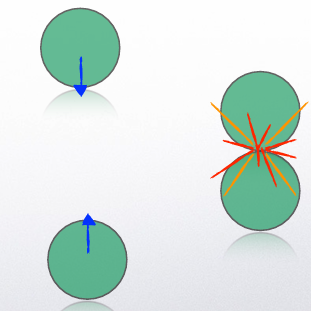
\includegraphics[width=0.3\linewidth]{photoMaterial/eventos_sistema_real.png}
  \end{center}
\end{frame}

\subsection{Modelo Matemático}
\begin{frame}{Modelo Matemático}
  \begin{itemize}
    \item Vuelo libre de las N particulas en un espacio 2D:
      \begin{itemize}
        \item $x_i(t) = x_i(0) + v_{x_i} t$
        \item $y_i(t) = y_i(0) + v_{y_i} t$
      \end{itemize}
    \item Calculo de tiempo de colision contra paredes:
      \begin{itemize}
        \item $t_{c} = \infty$ si $dv \cdot dr \geqslant 0$,
      \item $t_{c} = \infty$ si $d < 0$, siendo: $d = (dv \cdot dr)^2 - (dv \cdot dv)\cdot(dr \cdot dr - \sigma^2 )$,
        \item $\sigma = r_i + r_j$
        \item Colision con paredes espejan la velocidad en la normal de colision.
      \end{itemize}
  \end{itemize}
\end{frame}

% Colisiones entre particulas, formulas
\begin{frame}{Modelo Matemático}
  \begin{itemize}
    \item Calculo de impulso y velocidades post-colision de particulas:
      \begin{itemize}
        \item $J_x = J*dx/\sigma$
        \item $J_y = J*dy/\sigma$
        \item $J = \dfrac{2 m_i m_j}{m_i + m_j} \cdot \dfrac{dv \cdot dr}{\sigma}$
        \item $vx_i^d = vx_i^a + J_x/m_i$
        \item $vy_i^d = vy_i^a + J_y/m_i$
        \item $vx_j^d = vx_j^a - J_x/m_j$
        \item $vy_j^d = vy_j^a - J_y/m_j$
      \end{itemize}
    \item Coeficiente cuadratico medio: $<Z^2> = 2Dt$
  \end{itemize}
\end{frame}

% Implementación
\section{Implementación}
\begin{frame}{Implementación}
  \begin{itemize}
    \item Arquitectura del código.
    \item Pseudocódigo o UML.
  \end{itemize}
\end{frame}

% Simulaciones
\section{Simulaciones}
\begin{frame}{Simulaciones}
  \begin{itemize}
    \item Sistema particular simulado.
    \item Parámetros fijos y variables.
    \item Definición matemática de observables.
  \end{itemize}
\end{frame}

% Resultados
\section{Resultados}
\begin{frame}{Animaciones}
  % Aquí va la imagen de un frame representativo
  \includegraphics[width=0.7\linewidth]{ejemplo.png}
  
  \vspace{0.3cm}
  \footnotesize Link al video: \url{https://youtube.com/...}
\end{frame}

\begin{frame}{Evolución temporal del observable}
  \includegraphics[width=0.8\linewidth]{ejemplo_grafico.png}
  
  \vspace{0.3cm}
  Explicar el escalar característico (promedio, tasa, etc.).
\end{frame}

\begin{frame}{Input vs Observable}
  \includegraphics[width=0.8\linewidth]{ejemplo_resultados.png}
  
  \vspace{0.3cm}
  Mostrar promedios con barras de error.
\end{frame}

% Conclusiones
\section{Conclusiones}
\begin{frame}{Conclusiones}
  \begin{itemize}
    \item Conclusión 1 basada en los resultados.
    \item Conclusión 2…
  \end{itemize}
\end{frame}

% Cierre
\begin{frame}{}
  \centering
  \Huge ¡Gracias por su atención!
\end{frame}

\end{document}

